\subsection{Emergency Path Planning}\label{sub_section:tgt_path_planning}

\subsubsection{Cost Function}\label{sub_sub_section:tgt_cost_function}
The key objective is to reduce the downtime and cost of operation of the drone. This means both the cost of damage to the drone through crashing and the difficulty of retrieval need consideration. Considering the centre of each hexagon in the cost map as a node and modelling the probability of surviving half of a node node traversal between adjacent nodes as constant, $p$, the cost function of any path of length $D$ is shown in \ref{eq:cost function}. The specific $c_{crashing}$ and $c_{landing}$ can be defined by the ground operators for each classification. The ones used in testing are shown in \ref{tab:cost_values}.
\begin{equation}\label{eq:cost function}
    E(x) 
    = \sum_{n=1}^{D-1} c_{crashing}\bigl(x_n\bigr)\, (1-p) \,p^n 
    \;+\; c_{landing}\bigl(x_D\bigr)\, p^D
\end{equation}
\begin{table}[h]
    \centering
    \begin{tabular}{|c|c|c|c|c|}
    \hline
         \textbf{} & \textbf{Safe} & \textbf{Semi-Dangerous} & \textbf{Dangerous} & \textbf{Obstacle} \\
         \hline
         \textbf{$c_{landing}$} & 0 & 1 & 10 & 100 \\
         \textbf{$c_{crashing}$} & 10 & 10 & 100 & 1000\\
         \hline
    \end{tabular}
    \caption{Testing Costs}
    \label{tab:cost_values}
\end{table}

\subsubsection{Weather induced failure}\label{sub_sub_section:tgt_weather_failure}
\paragraph{Cause}
When a gust of wind exceeds the control capabilities of the drone it will cause an extreme disturbance and likely failure resulting in a crash. This is especially important to consider when their is an actuator fault due to the less aggressive control strategies deployed meaning that the maximum rejected gust becomes lower in magnitude and therefore more likely to occur. 
\paragraph{Gust Modelling}
Using forecasts and modelling as discussed in Section \ref{gust} we can model the probability that a gust exceeds the known maximum rejection gust speed for the current control gains per second, $\lambda$. From this we can calculate $p$ using Equation \ref{eq:p_calc}. The exact methods used to find $\lambda$ are an area of future work.
\begin{equation}\label{eq:p_calc}
    p = (1-\lambda)^{\frac{distance}{speed}}
\end{equation}

\subsubsection{Search Algorithms}\label{sub_sub_section:tgt_search}
\begin{algorithm}
\caption{Exhaustive Search}
\label{alg:search}
\begin{algorithmic}[1]
    \For{each Node $n$}
        \State $\textit{min\_cost} \gets \infty$
        \State $n.path\_cost$ = \Call{search}{$n$, $p$, $1$, $0$, $depth$, $\textit{min\_cost}$}
    \EndFor
    
    \Function{search}{$n$, $p$, $p\_alive$, $cost$, $depth$, \textbf{ref} $\textit{min\_cost}$}
        \State $\textit{current\_cost} \gets cost + p\_alive \cdot n.\textit{landing\_cost}$
        \If{$\textit{current\_cost} < \textit{min\_cost}$}
            \State $\textit{min\_cost} \gets \textit{current\_cost}$
        \EndIf
        \If{$depth = 0$ $\mathbf{or}$ $n.\textit{landing\_cost} = 0$ $\mathbf{or}$ $cost > \textit{min\_cost}$}
            \State \Return
        \EndIf
        \For{each $\textit{neighbour}$ in $n.\textit{neighbours}$}
            \State $p\_alive\_next \gets p\_alive \cdot p$
            \State $cost\_next \gets cost + p\_alive \cdot (1 - p) \cdot n.\textit{crashing\_cost}$
            \State \Call{search}{$\textit{neighbour}$, $p$, $p\_alive\_next$, $cost\_next$, $depth - 1$, $\textit{min\_cost}$}
        \EndFor
    \EndFunction
\end{algorithmic}
\end{algorithm}
\begin{algorithm}
    \caption{Smooth}
    \label{alg:flow}
\begin{algorithmic}[1]
    \While{not $Converged$}
        \State $Converged \gets TRUE$
        \For{each Node $n$}
            \For{each \textit{neighbour} in $n.\textit{neighbours}$}
                \State $\textit{movement\_cost} \gets n.\textit{crashing\_cost} \cdot \frac{1 - p}{2} +  \textit{neighbour}.\textit{crashing\_cost} \cdot \frac{p(1 - p)}{2}$
                \State $\textit{total\_cost} \gets \textit{movement\_cost} + p \cdot \textit{neighbour.path\_cost}$
                \If{$\textit{total\_cost} < n.\textit{path\_cost}$}
                    \State $n.\textit{path\_cost} \gets \textit{total\_cost}$
                    \State $Converged \gets FALSE$
                \EndIf
            \EndFor
        \EndFor
    \EndWhile
\end{algorithmic}
\end{algorithm}
\paragraph{Exhaustive Search}
The simplest algorithm is the recursive function shown in Algorithm \ref{alg:search}. There are steps taken to increase the efficiency, including pruning lines that already exceed the minimum cost as the cost is monotonic increasing and automatically terminating lines when they can land safely. However, the worst case time complexity remains $O(|V|6^{depth})$ as each node has 6 neighbours that get called recursively. To get guaranteed correct results it would require searching all paths as long as $|V|$ as costs cannot fall below 0 so it is never advantageous to revisit a node. Therefore, the worst case complexity for guaranteed optimal paths is $O(|V|6^{|V|})$. This is not usable for practical applications, therefore it requires a compromise to depth of search, no longer getting optimal path results.
\paragraph{Bellman-Ford}
To combat the issues with Algorithm \ref{alg:search}, I developed Algorithm \ref{alg:flow}. This algorithm smooths out the differences in path cost between neighbouring nodes following the Bellman-Ford algorithm. This guarantees correct answers when the nodes have fully converged. Bellman-Ford algorithms have a time complexity of $O(|E|\times |V|)$. In dense graphs this becomes  $O(|V|^3)$ however, we know $|E| \leq |V| \times 7$ as we are using hexagons can have an edge to 6 neighbours and a self edge indicating landing. Therefore the actual complexity is $O(|V|^2)$\cite{cormen2009}. This means it is practical to generate guaranteed optimal path results.

\subsubsection{Real-time application}\label{sub_sub_section:tgt_real_time}
\paragraph{Pre-Compute}
Carrying out memory and time complex operations on real-time hardware should always be avoided as operations require specific timings for optimal use. If all the values are pre-computed and uploaded to the device, the time and memory complexity becomes $O(1)$ which supports precise, timed operations. Within the path planning workflow, as much as possible should be pre-computed and simply accessed, however, if any algorithms are deployed they should be $O(1)$.
\paragraph{$p$ ranges}
While the value of $p$ can take any value between 0 and 1, there can be only 7 outputs for the next best move (going to each of the 6 neighbours or landing). Therefore, instead of creating a specific map for a specific value of $p$ on the flight controller you can pre-compute all the ranges of $p$ that would cause each of these outcomes. Then the device selects the option corresponding to its current $p$ value.
\paragraph{Deployment}
For a deployed algorithm consistent timings and a minimal memory footprint are essential. The algorithm \ref{alg:threshold} is used to select the next action based on the value of $p$ and the node $p$ ranges.
\begin{algorithm}[htbp]
  \caption{Threshold-Based Action Selection}
  \label{alg:threshold}
  \begin{algorithmic}[1]
    \Require Sorted threshold array \(\mathcal{P} = [p_1, p_2, \dots, p_6]\), associated actions \(\mathcal{A} = [a_1, a_2, \dots, a_6]\), input probability \(p\), default landing action \(a_{\textit{land}}\)
    \Ensure Selected action \(a\), GNSS coordinates \((\textit{lat}, \textit{lon})\)
    
    \State \(a \gets a_{\textit{land}}\) \Comment{Default to landing}
    \For{\(i = 1\) to \(n\)}
      \If{\(p < p_i\)}
        \State \(a \gets a_i\)
        \State \textbf{break}
      \EndIf
    \EndFor
    
    \State \((\textit{row}, \textit{col}) \gets \textit{GridCoordinates}(a)\)
    \State \((\textit{lat}, \textit{lon}) \gets \Call{ConvertToGNSS}{\textit{row}, \textit{col}}\)
    
    \State \Return \((a, \textit{lat}, \textit{lon})\)
  \end{algorithmic}
\end{algorithm}
\paragraph{Memory Management}
The memory on the \gls{MCU}s consists of Flash and \gls{SRAM}. Flash is static memory that has to be pre-loaded onto the board before each run whereas \gls{SRAM} is volatile but has faster access times. Therefore, waypoints, maps and gains are loaded into \gls{RAM} from the preset values in Flash before a flight. In addition, the flight controller's \gls{MCU} has \gls{ITCM} configured \gls{RAM} and \gls{DTCM} configured \gls{RAM}. \gls{DTCM} and \gls{ITCM} allow for precise timings when accessing data and instructions respectively and should therefore be used for looped processes including control loops and heading calculations. Whereas, for less timing critical actions or varying time operations such as actuator tests the regular \gls{SRAM} can be used. For the \gls{GNSS} module \gls{MCU} there is just Flash and \gls{SRAM} however, as it is a less complex operational loop this is sufficient. 
\begin{table}[h]
\centering
\begin{tabular}{ccccc} 
\toprule
\textbf{Device}&\textbf{Flash}&\textbf{SRAM}&\textbf{DTCM}&\textbf{ITCM}\\
 & (megabytes)& (kilobytes)& (kilobytes)& (kilobytes)\\
\midrule
STM32H743VGT6\tablefootnote{\url{https://www.st.com/en/microcontrollers-microprocessors/stm32h743vg.html}}&1&1000&128&64\\
MSPM0G3506SRHBR\tablefootnote{\url{https://www.ti.com/product/MSPM0G3506/part-details/MSPM0G3506SRHBR}}&0.128&64&-&-\\
\bottomrule
\end{tabular}
\caption{MCU Memory}
\label{tab:MCU_memory}
\end{table}

\paragraph{Memory Reduced Nodes}
Using a C implementation as shown in \ref{lst:node} it requires 56 bytes per node, therefore, for a 256 node map it requires 14.336 kilobytes of \gls{RAM}. This puts significant resolution limitations on the map. Therefore, the map should be stored in custom data structures that contain only as many bits as required. By using an indexed node array instead of pointers, 12 bit indexes can be used supporting 4096 nodes and 8 bits for probability values is sufficient. Lastly, the index of the node can be used to derive its location removing the relative values. This structure is shown in \ref{lst:reducednode} and with the above values and using guaranteed optimal number of thresholds and actions of 6 results in 16.5 bytes per node. However, the major drawback is that when moving away from from standard C data types bespoke bit operations are required increasing the development difficulty. 
\paragraph{Stop-Go Method}
The nature of the problem can be exploited using the strategy of the map having one option for the next move that above a probability threshold it goes to, and below that threshold it lands. This means that only one action and one threshold in the \ref{lst:reducednode} reduced node structure is needed resulting in a memory intensity of 4 bytes per node.
\begin{lstlisting}[caption={Implementated Node Structure},label={lst:node}]
struct Node {
    float rel_long, rel_lat;  // relative longitude and lattidue to reference point
    float p_values[6];        // Probability thresholds
    Node* actions[6];         // Points to the next node
};
\end{lstlisting}
\begin{lstlisting}[caption={Node Structure},label={lst:reducednode}]
struct Node {
    idx;           // Current Index Position
    p_values[];    // Probability thresholds
    actions[];     // Indexes of the next node
};
\end{lstlisting}
\subsubsection{Testing and Simulation}\label{sub_sub_section:tgt_testing_sims}
\paragraph{Testing}
Using 10 random satellite images from the Kharkiv region, 256 node cost maps were generated including visible obstacles and assumed regions of interest. Then starting at each node of the region of interest 20 separate trials are run using the different nodal structures. Their performances are calculated using random failures in line with $p$. The limitation of this method is the limited resolution and lack of actual real world data.
\paragraph{Reduced Nodes Performance Results}
The results in \ref{fig:Reduced Nodes} shows that the performances over the data set of the Stop-Go method is equivalent to the standard method. However, the Stop-Go method can no longer guarantee optimal results leaving them vulnerable to unforeseen situations and varying cost functions. Therefore, the reduced node \ref{lst:reducednode} should be implemented unless there are significant memory requirements.
\begin{figure}[htbp]
  \centering
  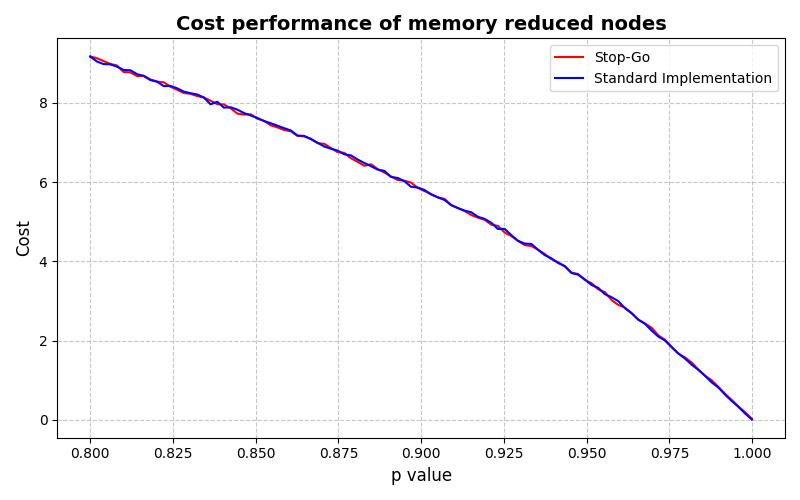
\includegraphics[width=1\textwidth]{figs/Thomas/Return To Safety/Reduced Nodes.png}
  \caption[Memory Reduced Nodes Performance]{Simulated results using Kharkiv test data based on method described in \ref{sub_sub_section:tgt_testing_sims} and the cost function in \ref{sub_sub_section:tgt_cost_function}}
  \label{fig:Reduced Nodes}
\end{figure}
